%! TEX root = main.tex

With the successful validation for the $Re=40$ cylinder flow, we were able to conduct the case study on the cylinder flow at $Re=200$.

\subsection{Configurations}

The computational domain is $[-8$, $25]$ $\times$ $[-8$, $8]$ for $x$ and $y$, and $t\in[0$, $200]$.
Other boundary conditions, initial conditions, and density were the same as those in section \ref{sec:val_2d_cylinder_re40}.
The non-dimensional kinematic viscosity is $0.005$ to make the Reynolds number $200$.

The PetIBM simulation was done with a grid resolution of $1485$ $\times$ $720$ and $\Delta t = \num{5e-3}$.
The hardware used and the configurations of the linear solvers were the same as described in section \ref{sec:val_2d_cylinder_re40}.

As for the PINN solvers, in addition to the steady and unsteady solvers, a third PINN solver was used: data-driven PINN.
The data-driven PINN solver is the same as the unsteady PINN solver but replaces the three initial condition losses ($L_4$ to $L_6$) with:
\begin{equation}\label{eq:data-driven-loss}
    \left\{
        \begin{array}{l}
            L_4 = u - u_{data}\\
            L_5 = v - v_{data}\\
            L_6 = p - p_{data}\\
        \end{array}
    \right.
    ,\text{ if }
    \begin{array}{l}
        \vec{x} \in \Omega \\
        t \in T_{data}
    \end{array}
\end{equation}
where subscript $data$ denotes the data from the PetIBM simulation.
$T_{data}$ denotes the time range where we feed the PetIBM simulation data to the data-driven PINN solver.
In this case, $T_{data} \equiv \left[125, 140\right]$.
The PetIBM simulation outputted transient snapshots every 1 second in simulation time, hence the data fed to the data-driven PINN solver consisted of 16 snapshots.
These snapshots contain around $3$ full periods of vortex shedding.
The total number of spatial-temporal points in these snapshots is around $\num{17000000}$, and we only used $\num{6400}$ every iteration, meaning each data batch was repeated approximately every $\num{2650}$ iterations.
Except for replacing the IC losses with a data-driven approach, all other loss terms in and the code in the data-driven PINN solver remain the same as the unsteady PINN solver.

Note that for the data-driven PINN solver, the PDE and boundary condition losses were evaluated only in $t\in[125$, $200]$ because we treated the PetIBM snapshots as if they were initial conditions.
Another note is the use of steady PINN solver.
The $Re=200$ cylinder flow is not expected to have a steady-state solution.
However, it is not uncommon to apply steady-state flow solver for unsteady flow for engineering purpose, especially two or three decades ago when computing power was not enough.

The MLP network used on all PINN solvers has 6 hidden layers and 512 neurons per layer.
The configurations of spatial-temporal points are the same as those in section \ref{sec:val_2d_cylinder_re40}.
The Adam optimizer is also the same, except that now we ran for \num{1000000} optimization iterations.
The parameters of the cyclical learning rate scheduler are now: $\eta_{low}=\num{1e-6}$, $\eta_{high}=\num{1e-2}$, $N_c=5000$, and $\gamma=\num{0.9999915}$.
The hardware used was one NVIDIA A100 GPU for all PINN solvers.

\subsection{Results}

The overall run times for the steady, unsteady, and data-driven PINN solvers are about 28 hours, 31 hours, and 33.5 hours using one A100 GPU.
The PetIBM simulation, on the other hand, took around 1.7 hours with a K40 GPU, which is 5-generation-behind in terms of the computing technology.

Figure \ref{fig:cylinder-re200-pinn-loss} shows the convergence history of all cases.
\begin{figure}
    \centering%
    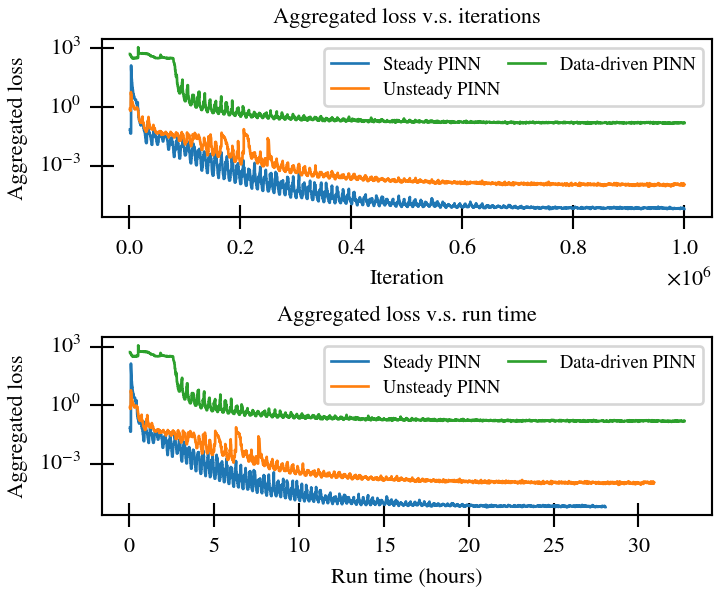
\includegraphics[width=0.95\columnwidth]{cylinder-2d-re200/loss-hist}%
    \caption{%
        Training convergence history of 2D cylinder flow at $Re=\num{200}$ w/ PINNs
    }
    \label{fig:cylinder-re200-pinn-loss}%
\end{figure}
It shows both the losses and the run times of the three PINN solvers.
As seen in section \ref{sec:val_2d_cylinder_re40}, the unsteady PINN solver converges to a higher total loss than the steady PINN solver does.
Also, the data-driven PINN solver converges to an even higher total loss.
However, it is unclear at this point if having a higher loss means the a higher prediction error in data-driven PINN because we replaced the initial condition losses with 16 snapshots from PetIBM and only ran the data-driven PINN solver for $t\in[125, 200]$.

Figure \ref{fig:cylinder-re200-drag-lift} shows the drag and lift coefficients versus simulation time.
\begin{figure}
    \centering%
    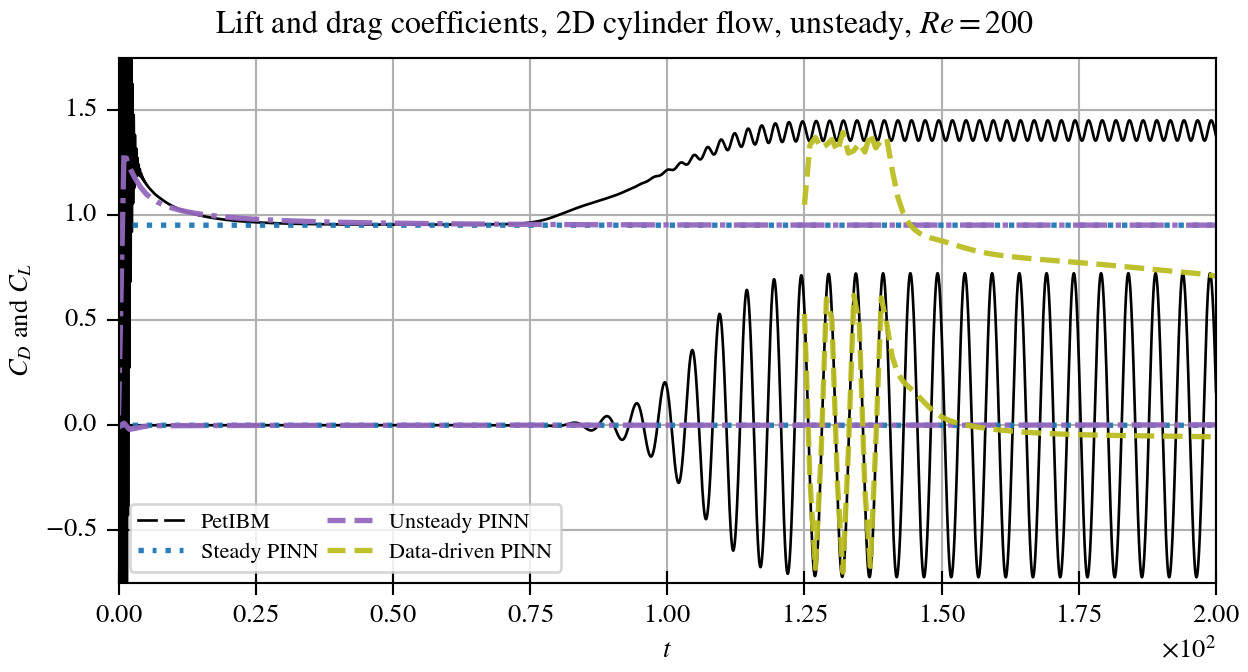
\includegraphics[width=0.95\columnwidth]{cylinder-2d-re200/drag-lift-coeffs}%
    \caption{%
        Drag and lift coefficients of 2D cylinder flow at $Re=\num{200}$ w/ PINNs
    }
    \label{fig:cylinder-re200-drag-lift}%
\end{figure}
The coefficients from the steady case is just a horizontal line since there is no time variable in this case.
The unsteady case, to our surprise, does not exhibit oscillation, meaning no vortex shedding, even though it fits well with the PetIBM result before vortex shedding (happens at about $t=75$).
Comparing the coefficients between the steady, unsteady, and PetIBM's values before shedding, we believe the unsteady PINN in this particular case behaves just like a steady solver.
This speculation is further supported by the values in table \ref{table:cylinder-2d-re200-cd}, in which we compare $C_D$ against literature of both unsteady and steady CFD simulations.
\begin{table}
    \centering%
    \begin{threeparttable}[b]
        \begin{tabular}{lcc}
            \toprule
            & $C_D$ \\
            \midrule
            PetIBM & 1.38   \\
            Steady PINN & 0.95 \\
            Unsteady PINN & 0.95 \\
            Deng et al., 2007\cite{deng_hydrodynamic_2007}\tnote{1} & 1.25 \\
            Rajani et al., 2009\cite{Rajani2009}\tnote{1} & 1.34 \\
            Gushchin \& Shchennikov, 1974\cite{gushchin_numerical_1974}\tnote{2} & 0.97 \\
            Fornberg, 1980\cite{fornberg_numerical_1980}\tnote{2} & 0.83 \\
            \bottomrule
        \end{tabular}%
        \begin{tablenotes}
            \footnotesize
            \item [1] Unsteady simulations.
            \item [2] Steady simulations.
        \end{tablenotes}
        \caption{%
            PINNs, 2D Cylinder, $Re=200$: validation of drag coefficients.%
            The data-driven case is excluded because it does not have an obvious periodic state nor a steady-state solution.%
        }%
        \label{table:cylinder-2d-re200-cd}
    \end{threeparttable}
\end{table}%
The $C_D$ obtained from the unsteady PINN is the same as the steady PINN and close to those steady CFD simulations.

As for the data-driven case, its temporal domain is $t\in[125$, $200]$, so the coefficients' trajectories start from $t=125$.
The result, again unexpected to us, only exhibits shedding in the timeframe with PetIBM data, i.e., $t\in[125$, $140]$.
This result also implies that data-driven PINNs may be more difficult to train, compared to data-free PINNs and regular data-only model fitting.
Even in the time range with PetIBM data, the data-driven PINN solver is not able to reach the given maximal $C_L$, and the $C_D$ is obviously off from the given data.
After $t=140$, the trajectories quickly fall back to the no-shedding pattern, though it still deviates from the trajectories of the steady and unsteady PINNs.
Combining the loss magnitude shown in figure \ref{fig:cylinder-re200-pinn-loss}, the deviation of $C_D$ and $C_L$ from the data-driven PINN may be caused by not enough training.
As figure \ref{fig:cylinder-re200-pinn-loss} shows data-driven PINN had already converged, other optimization techniques or hyperparameter tuning may be required to further reduce the loss.
Insufficient training only explains why the data-driven case deviates from the PetIBM's data in $t \in [125, 140]$ and from the other two PINNs for $t > 140$.
Even with a better optimization and eventually a lower loss, based on the trajectories, we do not believe the shedding will continue after $t=140$.

To examine how the transient flow develops, we visually compared several snapshots of the flow fields from PetIBM, unsteady PINN, and the data-driven PINN in figures \ref{fig:cylinder-re200-pinn-contours-u}, \ref{fig:cylinder-re200-pinn-contours-v}, \ref{fig:cylinder-re200-pinn-contours-p}, and \ref{fig:cylinder-re200-pinn-contours-omega_z}.
\begin{figure*}
    \centering%
    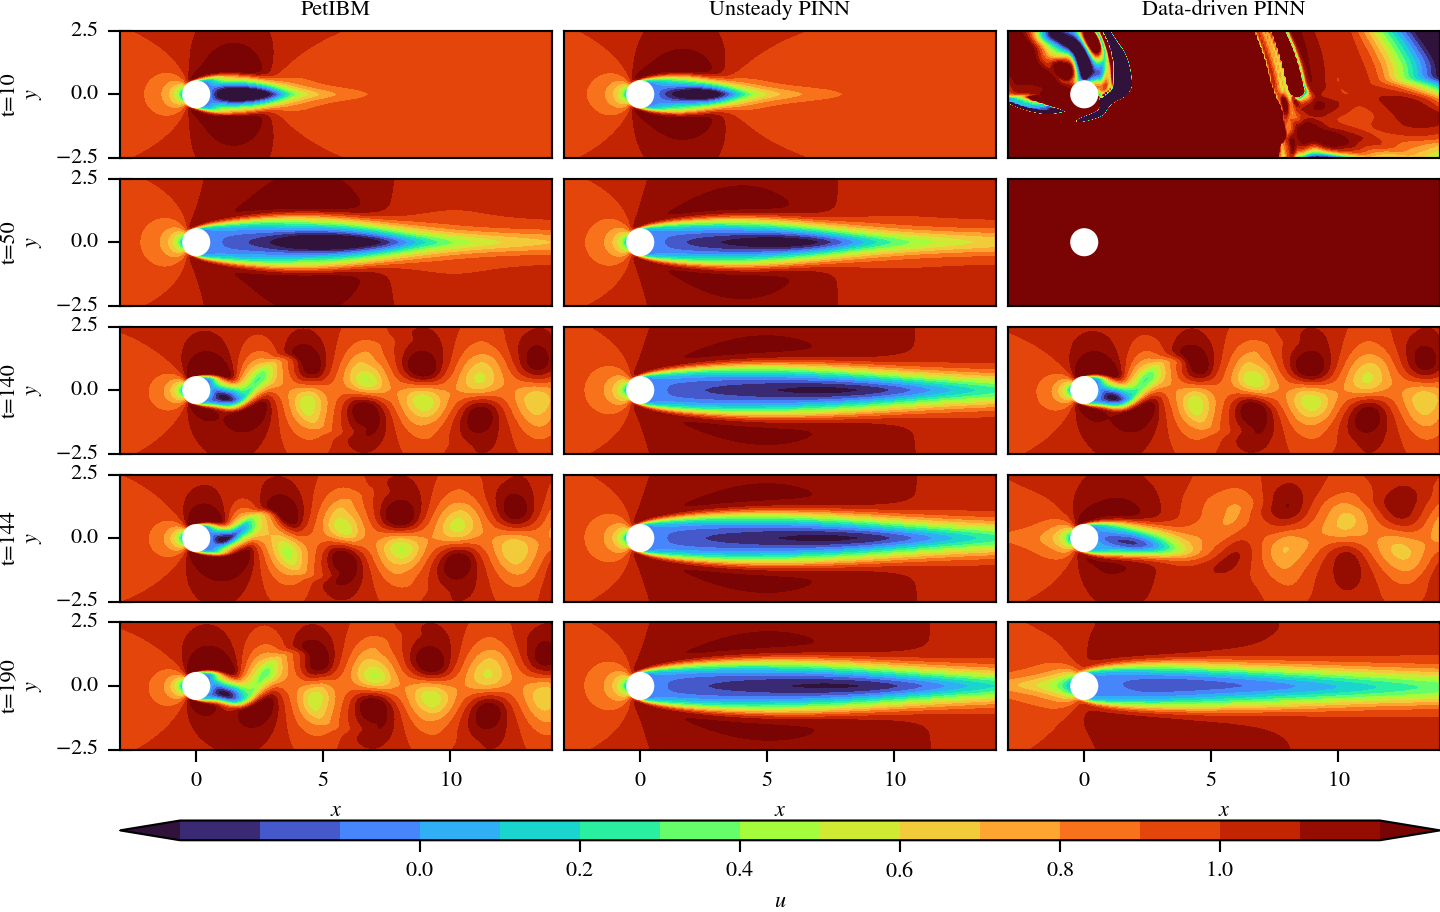
\includegraphics[width=0.95\textwidth]{cylinder-2d-re200/contour-comparison-u}%
    \caption{%
        $u$-velocity comparison of 2D cylinder flow of $Re=\num{200}$ between PetIBM, unsteady PINN, and data-driven PINN.
    }
    \label{fig:cylinder-re200-pinn-contours-u}%
\end{figure*}
\begin{figure*}
    \centering%
    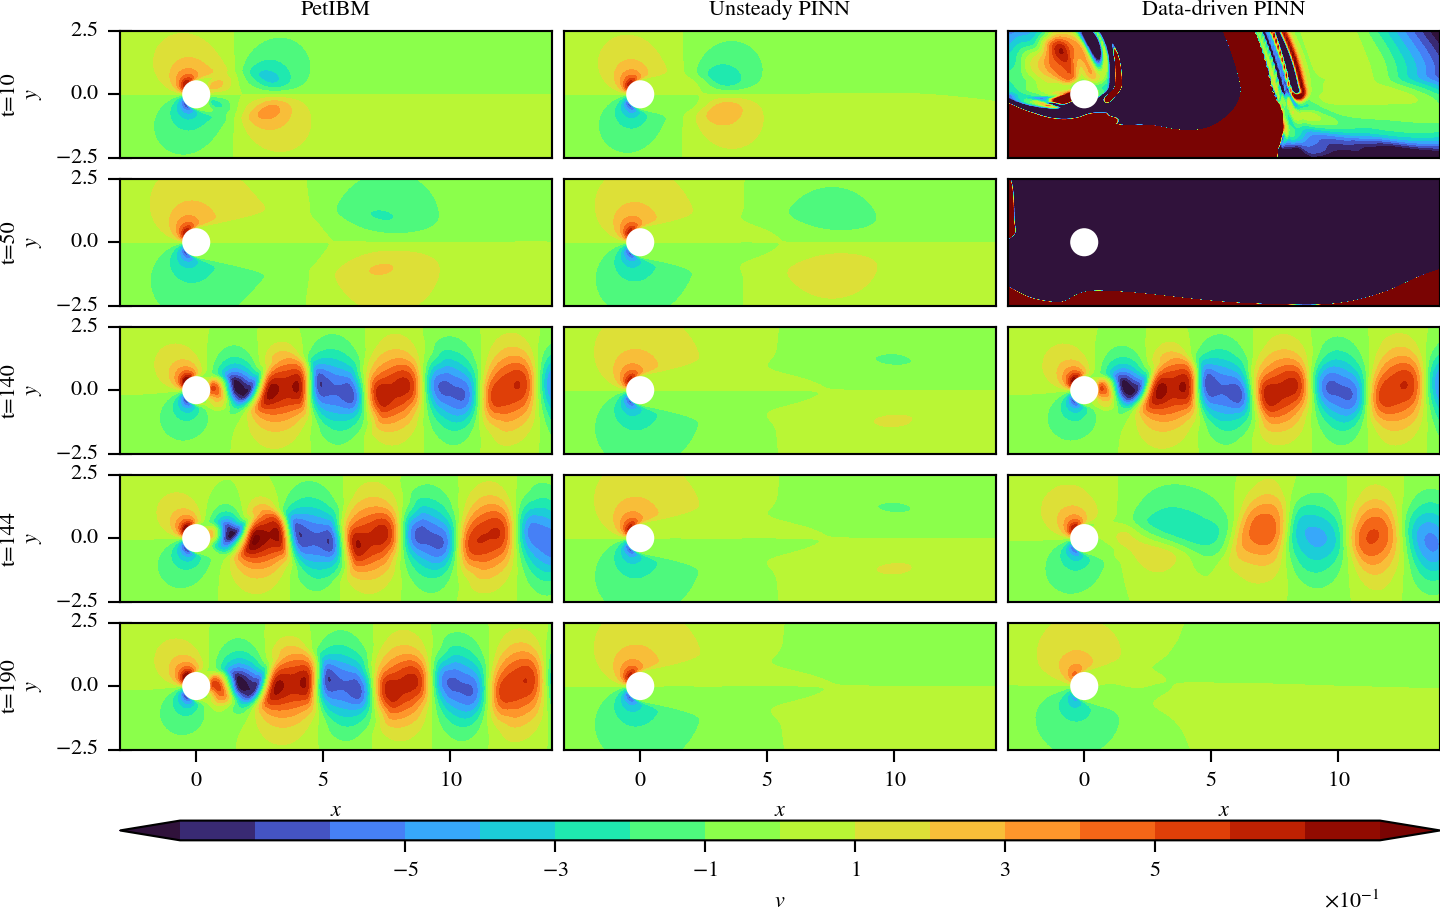
\includegraphics[width=0.95\textwidth]{cylinder-2d-re200/contour-comparison-v}%
    \caption{%
        $v$-velocity comparison of 2D cylinder flow of $Re=\num{200}$ between PetIBM, unsteady PINN, and data-driven PINN.
    }
    \label{fig:cylinder-re200-pinn-contours-v}%
\end{figure*}
\begin{figure*}
    \centering%
    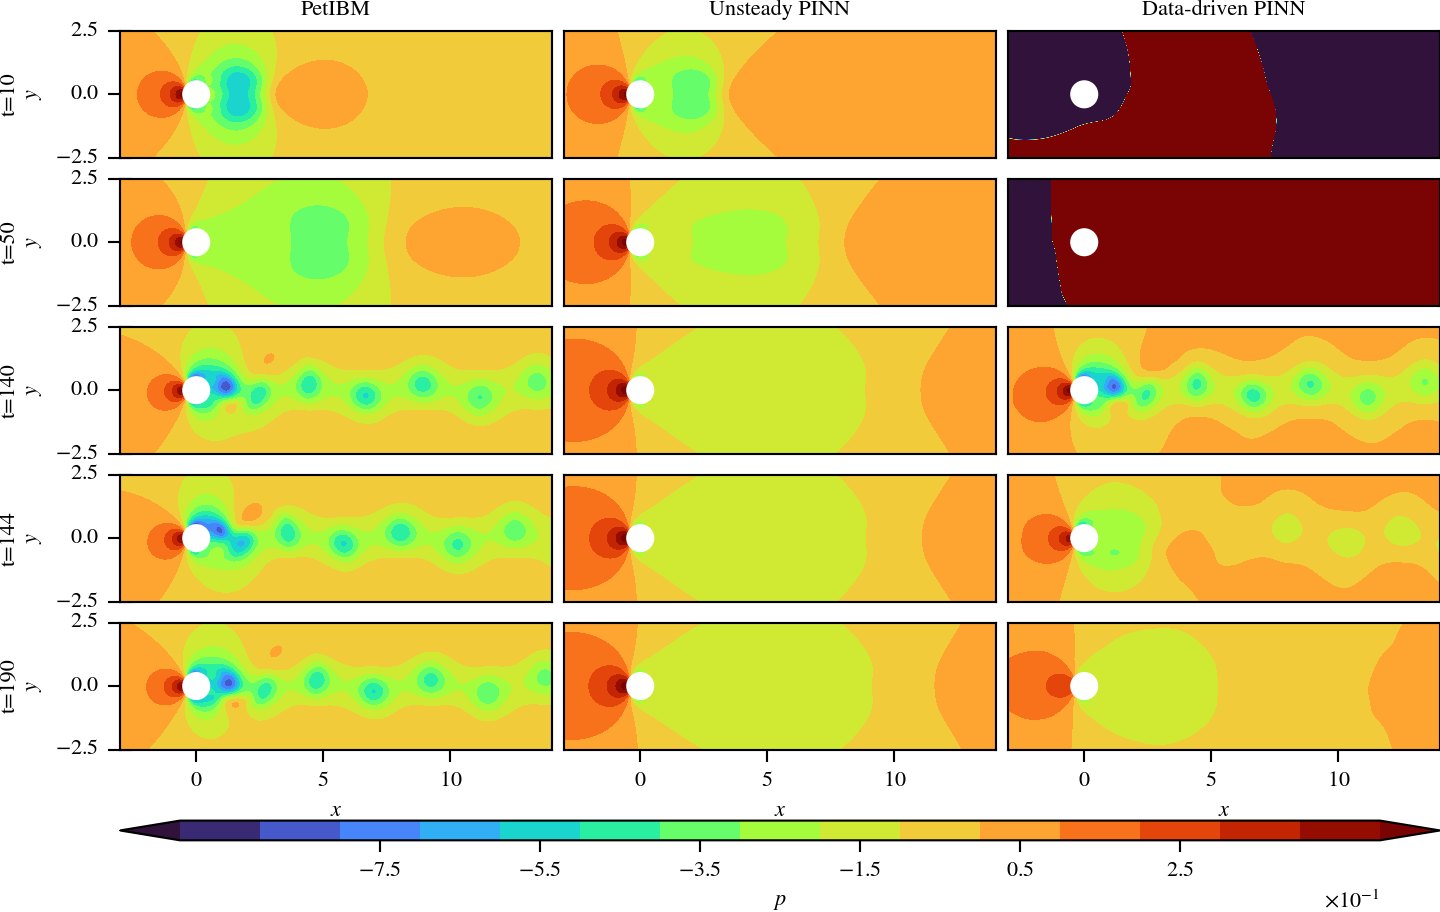
\includegraphics[width=0.95\textwidth]{cylinder-2d-re200/contour-comparison-p}%
    \caption{%
        Pressure comparison of 2D cylinder flow of $Re=\num{200}$ between PetIBM, unsteady PINN, and data-driven PINN.
    }
    \label{fig:cylinder-re200-pinn-contours-p}%
\end{figure*}
\begin{figure*}
    \centering%
    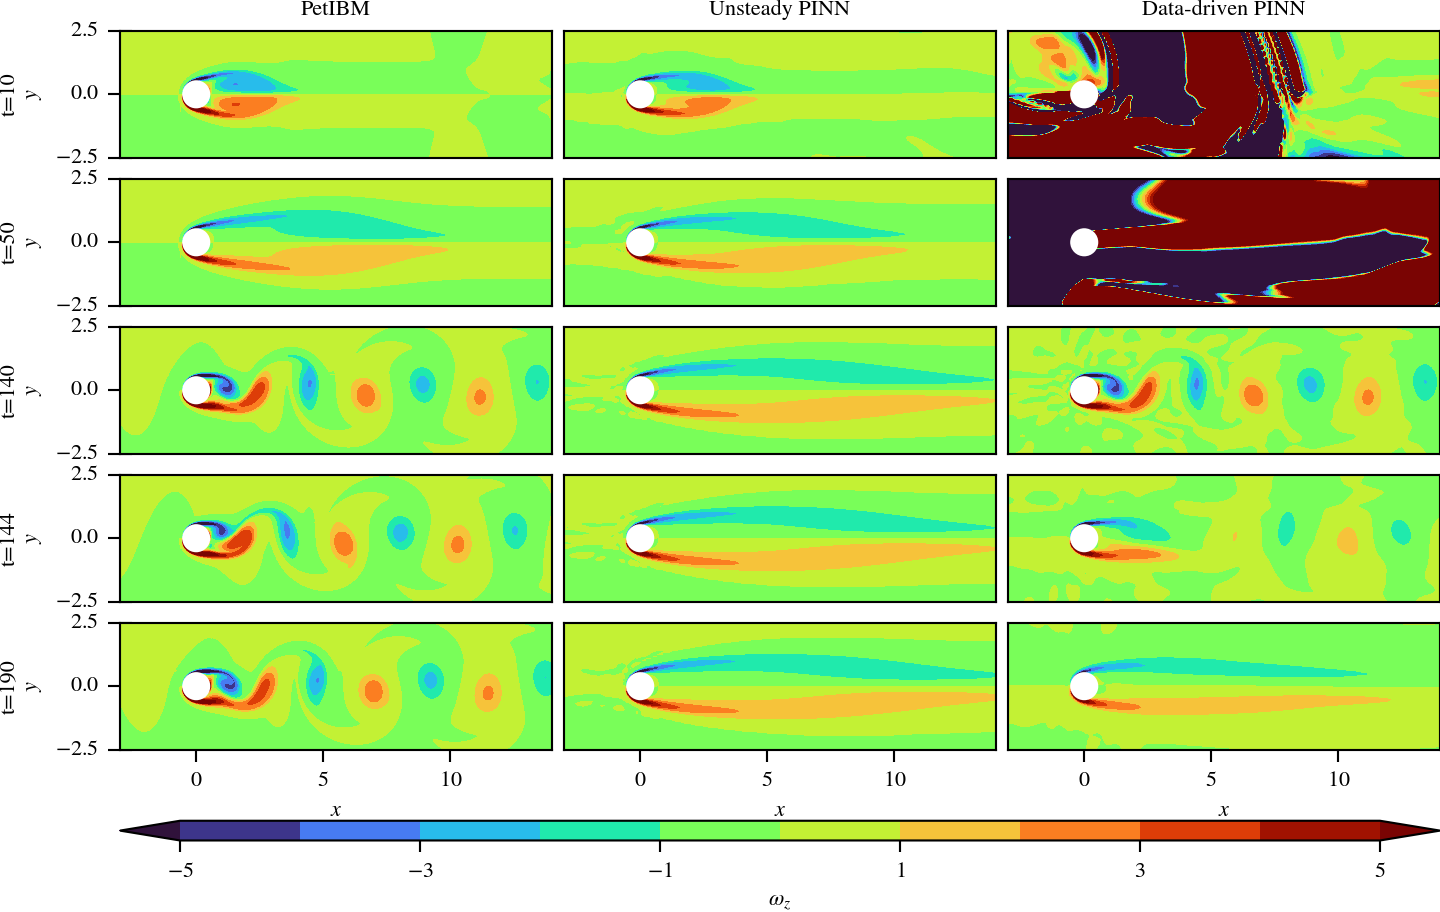
\includegraphics[width=0.95\textwidth]{cylinder-2d-re200/contour-comparison-omega_z}%
    \caption{%
        Vorticity ($\omega_z$) comparison of 2D cylinder flow of $Re=\num{200}$ between PetIBM, unsteady PINN, and data-driven PINN.
    }
    \label{fig:cylinder-re200-pinn-contours-omega_z}%
\end{figure*}
We also presented the flow contours from the steady PINN in figure \ref{fig:cylinder-re200-steady-pinn-contours} for reference.
\begin{figure}
    \centering%
    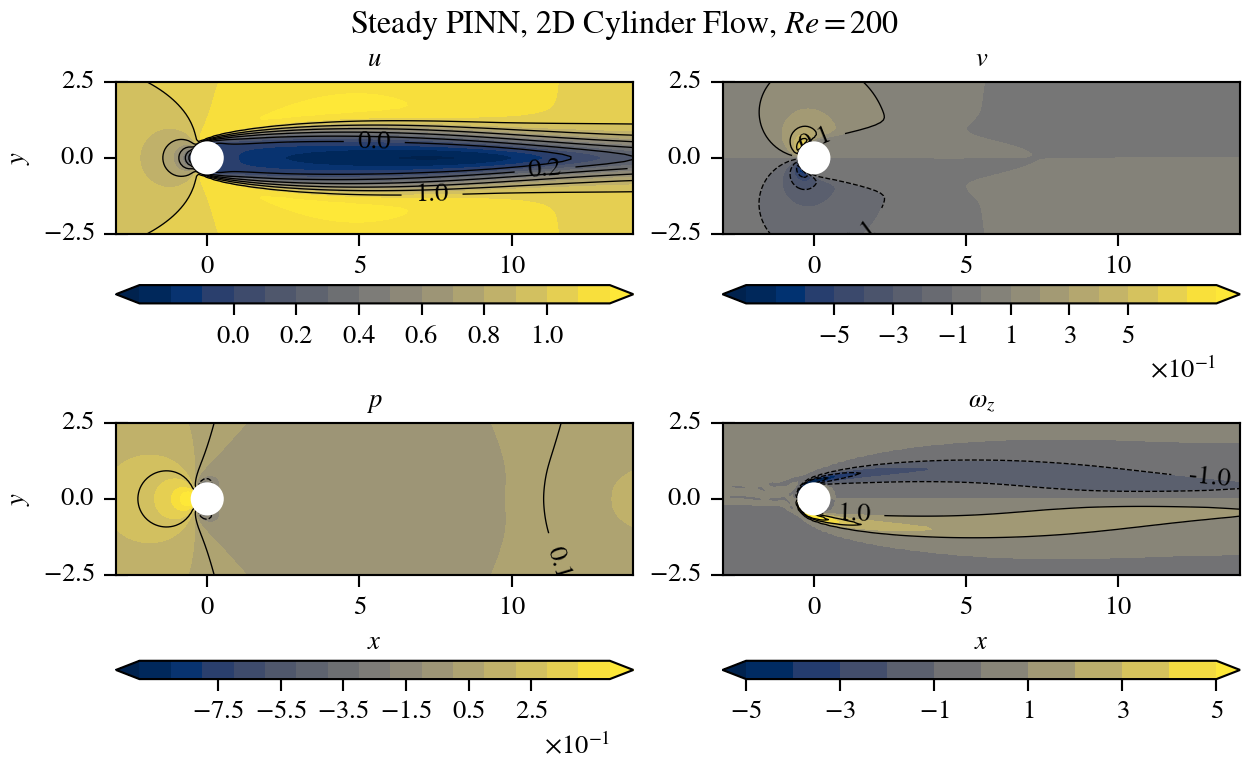
\includegraphics[width=0.95\columnwidth]{cylinder-2d-re200/contour-comparison-steady}%
    \caption{%
        Contours of 2D cylinder flow at $Re=\num{200}$ w/ steady PINN
    }
    \label{fig:cylinder-re200-steady-pinn-contours}%
\end{figure}

At $t=10$, we could see the wake is still developing, and the unsteady PINN visually matches PetIBM.
At $t=50$, the contours again confirm that the unsteady PINN matches the PetIBM simulation before shedding.
These observations verifies that the unsteady PINN is indeed solving unsteady governing equations.
The data-driven PINN does not show meaningful results because $t=10$ and $50$ are out of the data-driven PINN's temporal domain.
These results also indicates that data-driven PINN is not capable of extrapolating backward in time in dynamical systems.

At $t=140$, the shedding has already happened.
However, the unsteady PINN does not show any shedding.
Moreover, the unsteady PINN's contour is similar to the steady case in figure \ref{fig:cylinder-re200-steady-pinn-contours}.
$t=140$ is also the last snapshot we fed into the data-driven PINN for training.
The contour of the data-driven PINN at this time shows that it at least could qualitatively capture the shedding, which is expected.
At $t=144$, it is just $4$ unit time from the last snapshot being fed to the data-driven PINN.
However, the data-driven PINN has already stopped generating new vortices.
The existing vortex can be seen moving toward the boundary, and the wake is gradually restoring to the steady state wake.
Flow at $t=190$ further confirms that the data-driven PINN's behavior is leaning toward that of the unsteady PINN---which behaves like a steady state solver.
On the other hand, the solutions from the unsteady PINN for these times remain steady.

Figures \ref{fig:cylinder-re200-pinn-vort-gen} shows the vorticity from PetIBM and the data-driven PINN in the vicinity of the cylinder in $t \in [140, 142.5]$, which contains a half cycle of vortex shedding.
\begin{figure}
    \centering%
    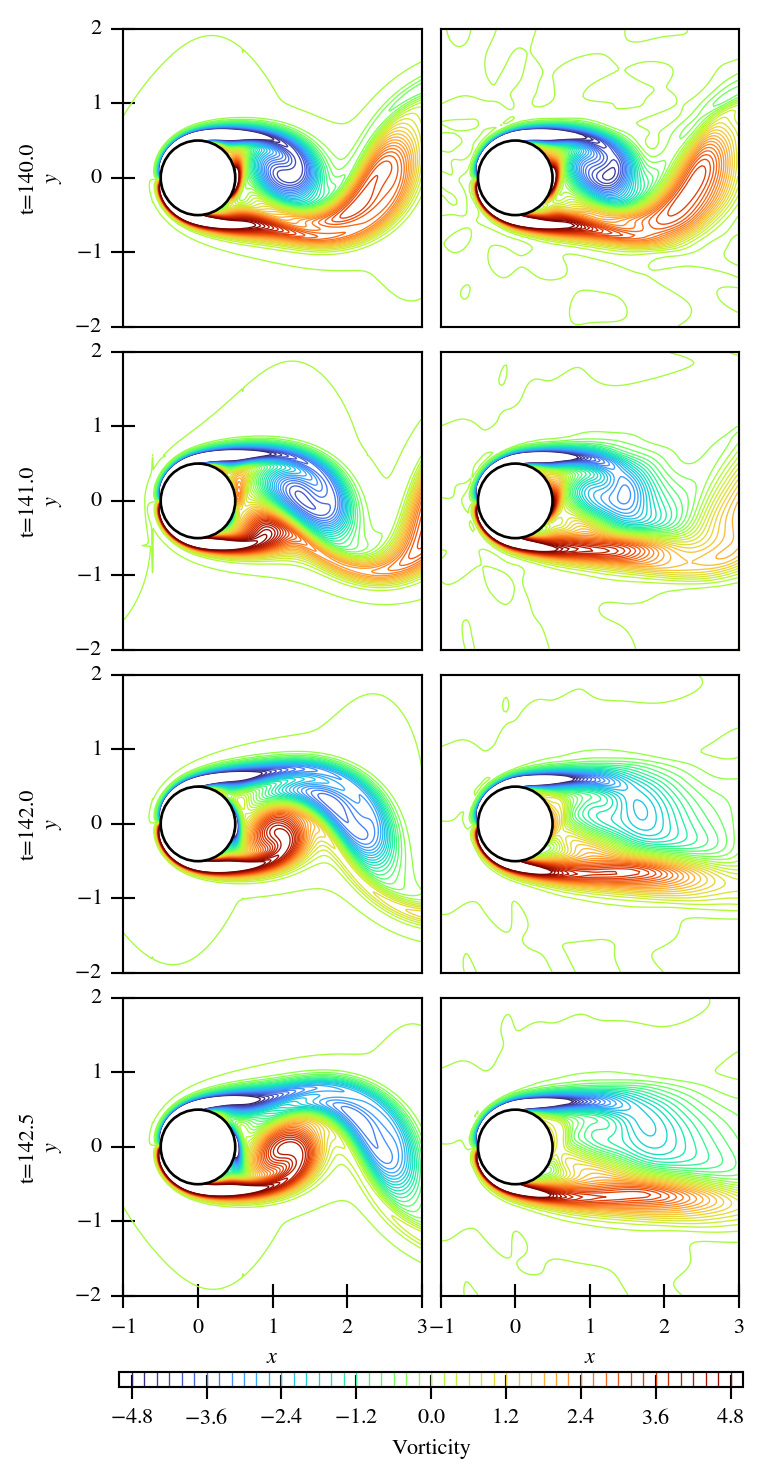
\includegraphics[width=\columnwidth]{cylinder-2d-re200/vorticity_z}%
    \caption{%
        Vorticity generation near the cylinder for 2D cylinder flow of $Re=\num{200}$ at $t=140$, $141$, $142$, and $142.5$ w/ data-driven PINNs.
    }
    \label{fig:cylinder-re200-pinn-vort-gen}%
\end{figure}
These contours compare how vorticity was generated right after we stopped feeding PetIBM data into the data-driven PINN.
These comparisons might shed some light on why the data-free PINN cannot generate vortex shedding and why the data-driven PINN stops to do so after $t=140$.

At $t=140$, PetIBM and the data-driven PINN show visually indistinguishable vorticity contours.
This is expected as the data-driven PINN has training data from PetIBM at this time.
At $t=141$ in PetIBM's results, the main clockwise vortex (the blue circular pattern in the domain of $[1, 2]\times[-0.5, 0.5]$) moves downstream.
It slows down the downstream's $u$ velocity and accelerates the latter's $v$ velocity in $y<0$.
Intuitively, we can treat the main clockwise vortex as a blocker that blocks the flow in $y<0$ and forces the flow to move upward.
The net effect is the generation of a counterclockwise vortex at around $x\approx 1$ and $y \in [-0.5, 0]$.
This new counterclockwise vortex further generates a small but strong secondary clockwise vortex on the cylinder surface in $y\in[-0.5, 0]$.
On the other hand, the result of the data-driven PINN at $t=141$ shows that the main clockwise vortex becomes more dissipative and weaker, compared to that in PetIBM.
It is possible that the main clockwise vortex is not strong enough to slow down the flow in $y<0$ nor to bring the flow upward.
The downstream flow in $y<0$ (the red arm-like pattern below the cylinder) thus does not change its direction and keeps going straight down in the $x$ direction.
In the results of $t=142$ and $t=142.5$ from PetIBM, the flow completes a half cycle.
That is, the flow pattern at $t=142.5$ is an upside down version of that at $t=140$.
The results from the data-driven PINN, however, do not have any new vortices and becomes more like steady flow.
These observations might indicate that the PINN is either diffusive or dissipative (or both).

Next, we examined the Q-criterion in the same vicinity of the cylinder in $t\in[140, 142.5]$ in figure \ref{fig:cylinder-re200-pinn-qcriterion}.
\begin{figure}
    \centering%
    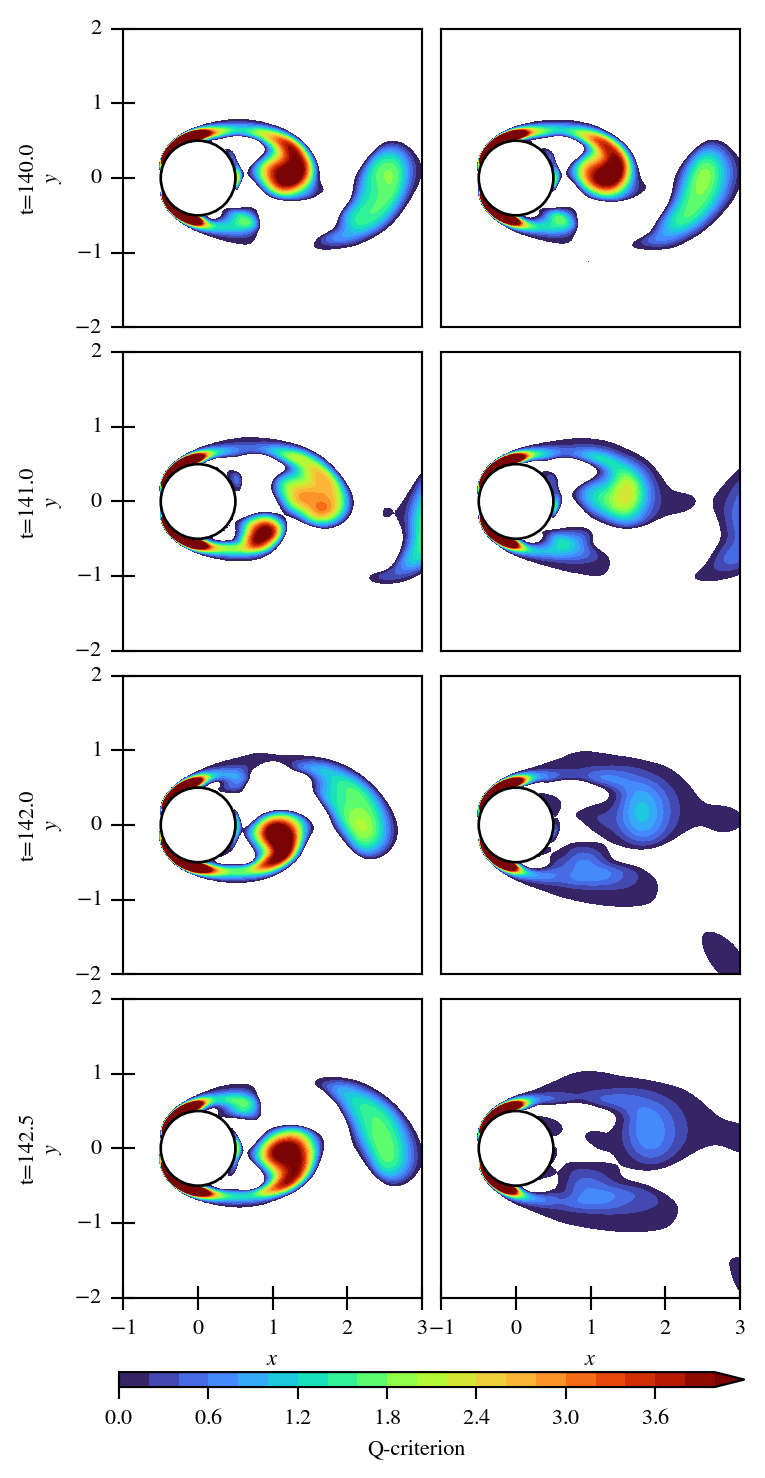
\includegraphics[width=\columnwidth]{cylinder-2d-re200/qcriterion}%
    \caption{%
        Q-criterion generation near the cylinder for 2D cylinder flow of $Re=\num{200}$ at $t=140$, $141$, $142$, and $142.5$ w/ data-driven PINNs.
    }
    \label{fig:cylinder-re200-pinn-qcriterion}%
\end{figure}
Q-criterion is defined as \cite{jeong_identification_1995}:
\begin{equation}
    Q \equiv \frac{1}{2}\left(\lVert \Omega \rVert^2 - \lVert S \rVert^2\right)
\end{equation}
where $\Omega\equiv\frac{1}{2}\left(\nabla\vec{u}-\nabla\vec{u}^\mathsf{T}\right)$ is the vorticity tensor;
$S\equiv\frac{1}{2}\left(\nabla\vec{u}+\nabla\vec{u}^\mathsf{T}\right)$ is the strain rate tensor;
$\nabla\vec{u}$ is the velocity gradient tensor.
A criterion $Q > 0$ identifies the vortex structure in fluid flow, that is, where the rotation rate is greater than the strain rate.

We observed that vortices in the data-driven PINN are diffusive and could be dissipative.
Moreover, judging by the locations of vortex centers, vortices also move slower in the PINN than in PetIBM.
The edges of the vortices move at a different speed from that of the vortex centers in the PINN.
This might be hinting the existence of the numerical dispersion in the PINN.

\subsection{Dynamical Modes and Koopman Analysis}

In this subsection, we conducted spectral analysis on the cylinder flow to extract frequencies embedded in the simulation results.
Fluid flow is a dynamical system, and how information (or signals) propagates in time plays an important role.
Information with different frequencies advances at different speeds in the temporal direction, and the superposition of information forms complicated flow patterns over time.
Spectral analysis reveals frequencies and corresponding information---which is called {\it dynamic modes} in fluid dynamics.
By comparing the dynamical modes against PetIBM, we examined how well/badly the data-driven PINN learned information with different frequencies.
Koopman analysis is an algorithm to achieve such spectral analysis for dynamical systems.
Please refer to {\it the method of snapshots} in reference \cite{chen_variants_2012} and \cite{rowley_spectral_2009} for the theory and the algorithms used in this work.

We analyzed the results from PetIBM and the data-driven PINN in $t\in$$[125$, $140]$, which contains about three full cycles of vortex shedding.
A total of $76$ solution snapshots were used from each solver.
The time spacing is $\Delta t = 0.2$.
The Koopman analysis would result in $75$ modes.
Since the snapshots cover three full cycles, we would expect only $25$ distinct frequencies and $25$ nontrivial modes---only $25$ out of $76$ snapshots are distinct.
However, this expectation only happens when the data are free from noise and numerical errors and when the number of three periods is exact.
We would see more than $25$ distinct frequencies and modes if the data were not ideal.
In $t \in [125, 140]$, the data-driven PINN was trained against PetIBM's data, so we expected to see similar spectral results between the two solvers.

To put it simply, each dynamical mode is identified by a complex number.
Taking logorithm on the complex number's absolute value gives a mode's growth rate, and the angle of the complex number corresponds to a mode's angular frequency.
Figure \ref{fig:cylinder-re200-koopman-eig-dist} shows the distributions of the dynamical modes on the complex plane.
\begin{figure}
    \centering%
    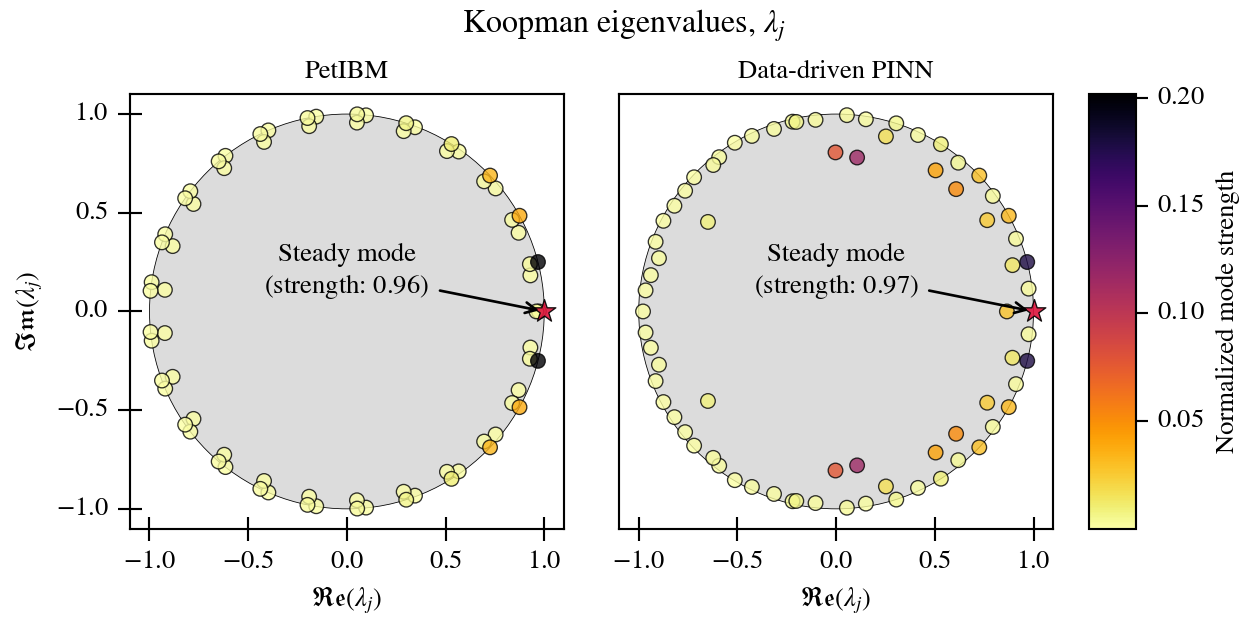
\includegraphics[width=\columnwidth]{cylinder-2d-re200/koopman_eigenvalues_complex}%
    \caption{%
        Distribution of the Koopman eigenvalues on the complex plane for 2D cylinder flow at $Re=\num{200}$.
    }
    \label{fig:cylinder-re200-koopman-eig-dist}%
\end{figure}
The color of each dot represents the normalized strength of the corresponding mode, which is also obtained from the Koopman analysis.
The star marker denotes the mode with a frequency of zero, i.e., a steady or time-independent mode.
This mode usually has much higher strength than others, so we excluded it from the color map and annotated its strength directly.
Koopman analysis delivers dynamical modes with complex conjugate pairs, so the modes are symmetric with respect to the real-number axis. 
A conjugate pair has an opposite sign in the frequencies in math but has the same physical frequency.

We also plotted a circle with a radius of one on each figure.
As flow has already reached a fully periodic regime, the growth rates should be zero because no mode can become stronger nor weaker.
In other words, all modes were expected to fall on this circle on the complex plane.
If a mode falls inside the circle, it has a negative growth rate, and its contribution to the solution diminishes over time.
Similarly, a mode falling outside the circle has a positive growth rate and becomes stronger over time.

On the complex plane, all PetIBM's modes (the left plot in figure \ref{fig:cylinder-re200-koopman-eig-dist}) fall onto the circle or close to the circle.
Though PetIBM's plot shows $75$---rather than $25$---distinct $\lambda_j$ and modes, modes are evenly clustered into 25 groups.
Each group has three modes, among which one or two modes fall on the circle, while the remaining one(s) falls inside but very close to the circle.
Modes within each group have a similar frequency, and the one precisely on the circle has significantly higher strength than other modes (if not all modes in the group are weak).
Due to the numerical errors in PetIBM's solutions, data in a vortex period are similar to but not exactly the same as those in another period.
The strong modes falling precisely on the circle may represent the period-averaged flow patterns and are the $25$ modes we expected earlier. 
The effect of numerical errors was filtered out from these modes.
We call these 25 modes primary modes and all other modes secondary modes.
Secondary modes are mostly weak and may come from the numerical errors in the PetIBM simulation.
The plot shows these secondary modes are slightly dispersive but non-increasing over time, which is reasonable because the numerical schemes in PetIBM are stable.

As for the PINN's result (the right in figure \ref{fig:cylinder-re200-koopman-eig-dist}), the mode distribution is not as structured as in PetIBM.
It is hard to distinguish if all 25 expected modes also exist in this plot.
However, we observed that at least the top 7 primary modes (the steady mode, two purple and 4 orange dots on the circle) also exist in the PINN's plot.
Secondary modes spread out more widely on and inside the circle, compared to the clustered modes in PetIBM.
We believe this means the PINN is more numerically dispersive and noisy.
The frequencies of many of these secondary modes do not exist in PetIBM.
So one possible source of these additional frequencies and modes may be the method of PINN itself.
It could be insufficient training or that the neural network itself inherently is dispersive. 
However, secondary modes on the circle are weak.
We suspect that their contribution to the solution may be trivial.

A more concerning observation is the presence of damped modes (modes that fall inside the circle). 
These modes have negative growth rates and hence are damped over time.
We believe these modes contribute significantly to the solution because their strengths are nontrivial.
The existence of the damped modes also means the PINN's predictions have more significant discrepancies from one vortex period to another vortex period, compared to the PetIBM's simulation.
In addition, the flow pattern in PINN would keep changing after $t=140$.
They may be the culprits causing the PINN's solution to quickly fall back to a non-oscillating solution for $t>140$.
We may consider these errors as numerical dissipation.
However, whether these errors came from insufficient training or were inherent in the PINN is unclear.

Note that the spectral analysis was done against data in $t\in[125, 140]$.
It does not mean the solutions in $t>140$ also have the same spectral characteristics: the flow system is nonlinear, but the Koopman analysis uses linear approximations \cite{rowley_spectral_2009}.

Figure \ref{fig:cylinder-re200-koopman-mode-strength} shows mode strengths versus frequencies.
\begin{figure}
    \centering%
    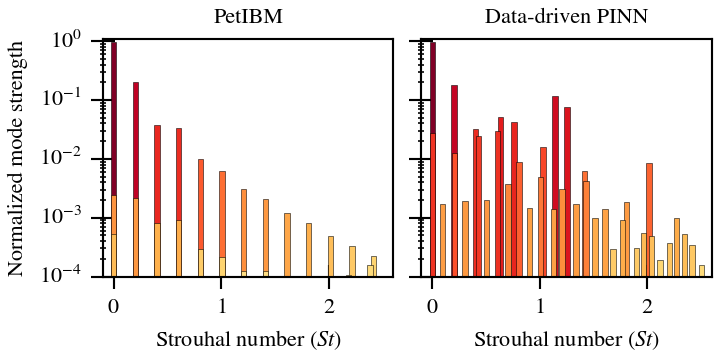
\includegraphics[width=\columnwidth]{cylinder-2d-re200/koopman_mode_strength}%
    \caption{%
        Mode strengths versus mode frequencies for 2D cylinder flow at $Re=\num{200}$.
        Note that we use a log scale for the vertical axis.
    }
    \label{fig:cylinder-re200-koopman-mode-strength}%
\end{figure}
The plots use nondimensional frequency, i.e., Strouhal number, in the horizontal axes. 
We only plotted modes with positive numerical frequencies for a concise visualization.
Plots in this figure also show the same observations in the previous paragraphs: the data-driven PINN is more dispersive and dissipative.

An observation that is now clearer from figure \ref{fig:cylinder-re200-koopman-mode-strength} is the strength distribution.
In PetIBM's plot, strengths decrease exponentially from the steady mode (i.e., $St=0$) to high-frequency modes.
One can deduce a similar conclusion from PetIBM's simulation result.
The vortex shedding is dominated by a single frequency (this frequency is $St\approx 0.2$ because $t\in[125, 140]$ contains three periods).
Therefore, the flow should be dominated by the steady mode and a mode with a frequency close to $St=0.2$.
We can indeed verify this statement from PetIBM's plot in figure \ref{fig:cylinder-re200-koopman-mode-strength}: the primary modes of $St=0$ and $St\approx 0.2$ are much stronger than others.
The strength of the immediately next mode, i.e., $St\approx 0.4$, drops in an order of magnitude. 
Note the use of the logarithm scale.
If we re-plot the figure using a regular scale, only $St=0$ and $St=0.2$ would be visible in the figure.

The strength distribution in the PINN's plot also shows that $St=0$ and $St\approx 0.2$ are strong.
However, they are not the only dominating modes.  
Some other modes also have strengths at around \num{e-1}.
As discovered in the previous paragraphs, these additional strong modes are damped modes.
We also observed that some damped modes have the same frequencies as primary modes.
For example, the secondary modes at $St=0$ and $St=0.2$ are damped modes.
Note that for $St=0$, if a mode is damped, then it is not a steady mode anymore because its magnitude changes with time, though it is still non-oscillating.

Table \ref{table:koopman-petibm} summarizes the top 4 modes (ranked in their strengths) in PetIBM's spectral result.
\begin{table}
    \begin{threeparttable}[b]
        \begin{tabular}{ccccc}
            \toprule
            $St$ & Strength & Growth Rate & Contours \\
            \midrule
            0     & 0.96 & 1.3e-7  & Figure \ref{fig:cylinder-re200-koopman-petibm-1st}\\
            0.201 & 0.20 & -4.3e-7 & Figure \ref{fig:cylinder-re200-koopman-petibm-2nd}\\
            0.403 & 0.04 & 1.7e-6  & Figure \ref{fig:cylinder-re200-koopman-petibm-3rd}\\
            0.604 & 0.03 & 2.7e-6  & Figure \ref{fig:cylinder-re200-koopman-petibm-4th}\\
            \bottomrule
        \end{tabular}%
        \caption{%
            2D Cylinder, $Re=200$: top 4 primary dynamic modes (sorted by strengths) for PetIBM%
        }%
        \label{table:koopman-petibm}
    \end{threeparttable}
\end{table}%
For reference, these modes' contours are provided in the appendex as denoted in the table.
The dynamic modes are complex-valued, and the contours include both the real and the imaginary parts.
Note the growth rates of these 4 modes are not exactly zero but around \num{e-6} and \num{e-7}.
We were unsure if we could treat them as zero at these orders of magnitude.
If not, and if they do cause the primary modes to be slightly damped or augmented over time, then we believe they also serve a reasonable explanation for the existence of the other 50 non-primary modes in PetIBM---to compensate for the loss or the gain in the primary modes.

Table \ref{table:koopman-pinn-primary} lists the PINN's top 4 primary modes, which are the same as those in table \ref{table:koopman-petibm}.
\begin{table}
    \begin{threeparttable}[b]
        \begin{tabular}{ccccc}
            \toprule
            $St$ & Strength & Growth Rate & Contours \\
            \midrule
            0     & 0.97 & -2.2e-6  & Figure \ref{fig:cylinder-re200-koopman-pinn-primary-1st}\\
            0.201 & 0.18 & -9.4e-6  & Figure \ref{fig:cylinder-re200-koopman-pinn-primary-2nd}\\
            0.403 & 0.03 &  2.3e-5  & Figure \ref{fig:cylinder-re200-koopman-pinn-primary-3rd}\\
            0.604 & 0.03 & -8.6e-5  & Figure \ref{fig:cylinder-re200-koopman-pinn-primary-4th}\\
            \bottomrule
        \end{tabular}%
        \caption{%
            2D Cylinder, $Re=200$: top 4 primary dynamic modes (sorted by strengths) for PINN%
        }%
        \label{table:koopman-pinn-primary}
    \end{threeparttable}
\end{table}%
Table \ref{table:koopman-pinn-damped} shows the top 4 secondary modes in the PINN's result.
\begin{table}
    \begin{threeparttable}[b]
        \begin{tabular}{ccccc}
            \toprule
            $St$ & Strength & Growth Rate & Contours \\
            \midrule
            1.142 & 0.12 & -0.24 & Figure \ref{fig:cylinder-re200-koopman-pinn-damped-1st}\\
            1.253 & 0.08 & -0.22 & Figure \ref{fig:cylinder-re200-koopman-pinn-damped-2nd}\\
            0.633 & 0.05 & -0.14 & Figure \ref{fig:cylinder-re200-koopman-pinn-damped-3rd}\\
            0.761 & 0.04 & -0.13 & Figure \ref{fig:cylinder-re200-koopman-pinn-damped-4th}\\
            \bottomrule
        \end{tabular}%
        \caption{%
            2D Cylinder, $Re=200$: top 4 damped dynamic modes (sorted by strengths) for PINN%
        }%
        \label{table:koopman-pinn-damped}
    \end{threeparttable}
\end{table}%
Corresponding contours are also included in the appendix and denoted in the tables for readers' reference.
The growth rates of the primary modes in the PINN's result are around \num{e-5} and \num{e-6}, slightly larger than that of PetIBM's.
If these orders of magnitude can not be deemed as zero, then these primary are slightly damped and dissipative, though the major source of the numerical dissipation may still be the secondary modes in table \ref{table:koopman-pinn-damped}.

% vim:ft=tex: